%! TEX root = ../../master.tex
Wir wollen nun noch den Satz von \nameref{thm:seifert-van-kampen} beweisen, den wir noch einmal wiedergeben:

\lecture[Beginn des Beweises von Seifert van Kampen.]{Do 08 Jul 2021}[22]{}[Ende der Vorlesung]

\restatetheorem*{ThmSeifertVanKampen}

\begin{proof}
    Das Inklusionsdiagramm induziert - da $\pi_1$ ein Funktor ist - ein kommutatives Diagramm von Gruppenmorphismen
    \[
        \begin{tikzcd}[anchor=center]
        U_3 \ar[swap, phantom]{d}[rotate=-90]{\subset } \ar[phantom]{r}{\subset } & U_1 \ar[phantom]{d}[rotate=-90]{\subset } \\
        U_2 \ar[swap, phantom]{r}{\subset } & X
    \end{tikzcd}
    \quad \stackrel{\pi_1}{\leadsto} \quad
    \begin{tikzcd}[anchor=center]
        \pi_1( U_3 ,x_0)\ar[swap]{d}{\psi _2} \ar{r}{\psi _1} &\pi_1( U_1,x_0) \ar{d}{\varphi_1} \\
        \pi_1(U_2,x_0) \ar[swap]{r}{\varphi_2} & \pi_1(X,x_0)
    \end{tikzcd}
    \]
Wir wollen zeigen, dass das rechte Diagramm ebenfalls ein Pushout ist, und wissen bereits, dass Pushouts in Gruppen durch das amalgisierte Produkt gegeben sind, wir wollen also einen Isomorphismus
\[
    \pi_1(U_1,x_0) \amalgprod_{\pi_1(U_3,x_0)} \pi_1(U_2,x_0) \twoheadrightarrow \pi_1(X,x_0)
\] 
konstruieren. Notieren nun 
\[
    \Psi \colon \pi_1(U_1,x_0) \amalgprod \pi_1(U_2,x_0) \to \pi_1(X,x_0)
\] 


\begin{claim}
    Es ist $\Psi$ surjektiv.
\end{claim}
\begin{subproof}
    
    Da $I$ kompakt ist, existiert  für jeden Weg $[w] \in \pi_1(X,x_0)$ ein $k\in \mathbb{N}$, sodass
    \[
w_l \coloneqq         w|_{\left[ \frac{l}{k}, \frac{l+1}{k} \right) } \subset U_i
    .\] 
    für alle $l$. Für alle  $l\in \left \{1,k-1\right\}$ wähle einen Weg $v_l$ von  $w\left( \frac{l}{k} \right) $ nach $x_0$ in 
    \[
    \begin{cases}
        U_3 & \text{falls } w\left( \frac{l}{k} \right) \in U_3 \\
        U_1 & \text{falls } w\left( \frac{l}{k} \right) \not\in U_2 \\
        U_2 & \text{falls } w\left( \frac{l}{k} \right)  \not\in U_1
    \end{cases}
    .\] 
    Beachte hierzu, dass wir im ersten Fall natürlich verwenden, dass $U_3$ wegzusammenhängend ist. Setze $w_l \coloneqq  w|_{\left[ \frac{l}{k}, \frac{l+1}{k} \right] }$ für $l=0,\ldots,k-1$ als die Teilstücke von $w$, dann können wir umschreiben:
    \begin{IEEEeqnarray*}{rCl}
        [w] & = & w_0\star w_2\star \ldots \star w_{l-1} \\
            & = & w_0\star (v_1\star v_1^{-1}) \star w_1 \star (v_2\star v_2^{-1}) \star \ldots \star w_{l-1} \\
            & = & [w_0\star v_1] \star [v_1^{-1} w_1 v_2] \star \ldots \star [v_{k-1}^{-1}w_{k-1}]
    \end{IEEEeqnarray*}
    und jeder der geklammerten Wege verläuft nun nach Konstruktion in einem der $U_i$. In der unteren Zeile handelt es sich also nun um eine Verkettung aus Elementen von $\pi_1(U_1,x_0)$ und $\pi(U_2,x_0)$, also genau um ein Element aus dem freien Produkt der beiden Gruppen.
\end{subproof}

\lecture[Beweis von Seifert-van-Kampen.]{Di 13 Jul 2021}[23]{Beweis des Satzes von Seifert-van-Kampen}

    Wir interessieren uns natürlich im folgenden für den Kern von $\Psi$ und wollen zeigen, dass dieser genau von den Relationen der Einbettungen  $\psi_1, \psi_2$ erzeugt wird. Setze also
    \begin{equation*}
    F: \left| \begin{array}{c c l} 
        \pi_1(U_3,x_0) & \longrightarrow & \pi_1(U_1,x_0) \amalgprod \pi_1(U_2,x_0) \\
        r & \longmapsto &  \psi _1(r) \psi _2(r)^{-1} 
    \end{array} \right.
    \end{equation*}
    \begin{warning}
        $F$ ist kein Homomorphismus, sondern erstmal nur eine Abbildung.
    \end{warning}
    \begin{claim}
        Der Kern von $\Psi$ ist der normale Abschluss des Bildes von  $F$, d.h.
         \[
             \ker \Psi = \overline{F(\pi_1(U_3,x_0))}
        \] 
    \end{claim}

    \begin{notation*}
        Seien $a,b$ Wegen in  $X$ (an  $x_0$), dann schreiben wir
        \begin{itemize}
            \item $a\sim _{U_i} b \coloneqq $ $a,b$ sind Wege in $U_i$ und homotop in  $U_i$
            \item  $a\sim _{X} b \coloneqq $ $a,b$ sind homotop in $X$. 
        \end{itemize}
        Sei $a$ eine Schleife an  $x_0$, dann notiere mit
        \begin{itemize}
            \item $[a]_{U_i\coloneqq }$ die Klasse von $a$ in  $\pi_1(U_i, x_0)$, und meine implizit, dass $a$ in  $U_i$ liegt.
            \item $[a]_X\coloneqq $ die Klasse von $a$ in  $\pi_1(X,x_0)$
        \end{itemize}
    \end{notation*}
    Damit ergibt sich z.B.
    \[
        \psi _1([a]_{U_3}) = [a]_{U_1} \qquad \psi _2([a]_{U_3}) = [a]_{U_2}
    \] 
    Für die verschiedenen Typen von Multiplikation notieren wir
    \begin{itemize}[-]
        \item $\bullet$ für die Wegemultiplikation in den Fundamentalgruppen  $\pi_1(U_i,x_0)$ oder $\pi_1(X,x_0)$
        \item $\amalgprod$ für die Multiplikation in  $\pi_1(U_1,x_0) \amalgprod \pi_1(U_2,x_0)$.
    \end{itemize}
    Damit ergibt sich z.B:
    \[
        [a]_{U_1} \amalgprod [b]_{U_2} \amalgprod [c]_{U_2} = [a \bullet b] \amalgprod  [c]_{U_2} \in \pi_1(U_1,x_0) \amalgprod  \pi_1(U_2,x_0)
    \]
    oder auch
    \begin{IEEEeqnarray*}{rCl}
    & &    \Psi([a_1]_{U_1} \amalgprod  [a_2] _{U_2} \amalgprod  \ldots \amalgprod  [a_{m}]_{U_2})  \\
    & = & \psi _1 [a_1]_{U_1} \bullet \psi_2 [a_2] _{U_2} \bullet  \ldots \bullet  \psi _2 [a_m] _{U_2}0\\
    & = & [a_1]_X \bullet  [a_2] _X \bullet  \ldots \bullet  [a_m] _X \\
    & = & [a_1 \bullet  \ldots \bullet a_m]_X
    \end{IEEEeqnarray*}

    Sei nun
    \[
        N\coloneqq  \overline{F(\pi_1(U_3,x_0))}
    \] 
    der normale Abschluss des Bildes von $F$. Wir wollen also  $N = \ker \Psi$ zeigen.

     \begin{claim}
        Es ist $N \leq  \ker \Psi$.
    \end{claim}
    \begin{subproof}
        Es genügt zu zeigen, dass $F(\pi_1(U_3,x_0)) \subset \ker \Psi$ ist, denn $\ker \Psi$ ist normal. 

        Sei nun $[a]_{U_3}\in \pi_1(U_3,x_0)$. Dann ist
        \begin{IEEEeqnarray*}{rCl}
            \Psi \circ  F([a]_{U_3}) & = & \Psi (\varphi_1([a]_{U_3}) \amalgprod \varphi_2([a]_{U_3})^{-1} \\
                                     & = & \Psi ([a]_{U_1} \star [a]_{U_2}^{-1}) \\
                                     & = & \psi _1([a]_{U_1}) \bullet \psi _2([a]_{U_2}^{-1}) \\
                                     & = & [a]_X \bullet [a]_X^{-1} \\
                                     & = & [a \bullet a^{-1}]_X \\
                                     & = & 1
        \end{IEEEeqnarray*}
    \end{subproof}

    \begin{claim}
        Es ist auch $\ker \Psi \leq  N$.
    \end{claim}
    \begin{subproof}
        Sei
        \[
            \gamma = [a_1]_{U_1} \amalgprod [a_2]_{U_2}\amalgprod \ldots \amalgprod [a_k]_{U_2} \in  \pi_1(U_1,x_0) \amalgprod  \pi_1(U_2,x_0)
        \] 
        mit $\Psi(γ) = 1$, also
        \[
            [a_1 \bullet  \ldots \bullet  a_k]_X = 1
        \] 
        Also finden wir eine Homotopie
        \[
        a_1 \bullet \ldots \bullet  a_k \sim _X c_{x_0}
        \] 
        zur konstanten Schleife an $x_0$. Sei 
        \[
            H\colon  [0,1] \times  [0,1] \to X
        \] 
        eine solche Homotopie (relativ Endpunkten) von $a_1\bullet \ldots\bullet a_k$ nach $c_{x_0}$. Wir unterteilen die Homotopie nun in kleinere Einheitsquadrate, d.h. setze
        \[
        S_{ij} \coloneqq  \left[ \frac{i-1}{n}, \frac{i}{n} \right] \times \left[ \frac{j-1}{n}, \frac{j}{n} \right] 
        \] 
        \[
    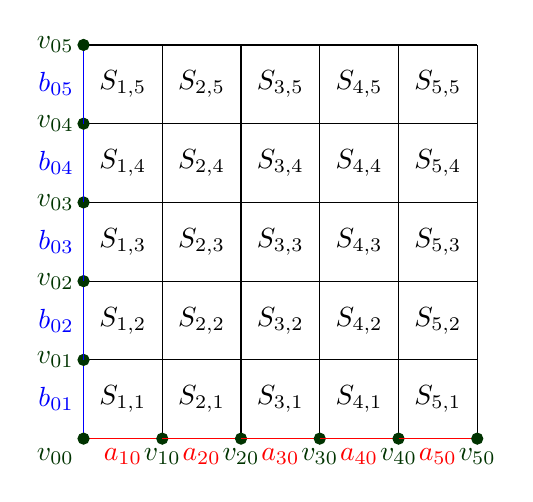
\begin{tikzpicture}
        \draw (0,0) grid (5,5);
        \foreach \x in {1,2,3,4,5} {
            \foreach \y in {1,2,3,4,5} {
                \node at (\x-0.5, \y-0.5) {$S_{\x, \y}$};
            }
        }
        \foreach \x in {1,2,3,4,5} {
            \draw[red] (\x-1,0) -- (\x,0) node[midway, anchor=north] {$a_{\x 0}$};
            \draw[green!20!black, fill] (\x,0) circle (2pt) node[anchor=north] {$v_{\x 0}$};
        }
        \foreach \y in {1,2,3,4,5} {
            \draw[blue] (0,\y-1) -- (0,\y) node[midway, anchor=east] {$b_{0\y}$};
            \draw[green!20!black, fill] (0,\y) circle (2pt) node[anchor=east] {$v_{0\y}$};
        }
        \draw[green!20!black, fill] (0,0) circle (2pt) node[anchor= north east] {$v_{00}$};
    \end{tikzpicture}
\]
Da $I^2$ kompakt ist, $\exists n\in \mathbb{N}$, sodass jedes der $S_{ij}$ durch $H$ in  $U_1$ oder $U_2$ abgebildet wird.

Wir wählen zudem $n$ groß genug, sodass die Endpunkte von  $a_i$ jeweils von der Form  $\frac{i'}{n}$ sind für ein $i'\in \mathbb{N}$. Setze nun
\[
    a_{ij} \coloneqq  H|_{\left[ \frac{i-1}{n}, \frac{i}{n} \right] \times \left \{\frac{j}{n}\right\} } \qquad b_{ij} = H|_{\left \{\frac{i}{n}\right\} \times \left[ \frac{j-1}{n}, \frac{j}{n} \right] } \qquad v_{ij} = H\left( \frac{i}{n}, \frac{j}{n} \right) 
\] 
Also ist nach Definition
\begin{IEEEeqnarray*}{rCl}
    H|_{[0,1]\times 0} &=& a_1\cdot a_2\cdot \ldots\cdot  \\
                       & = & \underbrace{(a_{10} \bullet a_{20} \bullet \ldots\bullet a_{p_0})}_{a_1} \bullet (a_{p+1,0}\ldots) \ldots \underbrace{(a_{q_0}\bullet \ldots\bullet a_{r_0})}_{a_k}
\end{IEEEeqnarray*}
Also gitl in $\pi_1(U_1,x_0) \amalgprod \pi_1(U_2,x_0)$ gerade:
\[
    \gamma = [a_{10}\bullet  \ldots \bullet a_{p_0}]_{U_1} \amalgprod  [a_{p+1,0} \bullet \ldots] \amalgprod  \ldots \amalgprod  [a_{q_0} \bullet \ldots ]_{U_2}
\] 
Allerdings sind nun die einzelnen $i_{ij}$ noch nicht zwangsweise Schleifen an $x_0$, weil wir die ursprünglichen Schleifen $a_i$ ja 'zerschnitten' haben. Wir sehen uns nun ein typischen der Quadrate  $S_{ij}$, bzw. das zugehörige Bild in $X$, an. Siehe hierzu \autoref{fig:ausschnitt-quadrat-in-x-seifert-van-kampen}.

Wähle nun Wege $h_{ij}$ von $x_0$ nach $v_{ij}$, sodass
\begin{itemize}
    \item falls $v_{ij} \in U_l$, wähle $h_{ij} \subset U_l$ für $l = 1,2,3$.
    \item Falls $v_{ij} = x_0$, so wähle $h_{ij} = c_{x_0}$ konstant.
\end{itemize}

\begin{figure}[ht]
    \centering
    \incfig{ausschnitt-quadrat-in-x-seifert-van-kampen}
    \caption{Ausschnitt Quadrat in X Seifert van Kampen}
    \label{fig:ausschnitt-quadrat-in-x-seifert-van-kampen}
\end{figure}


Jetzt setzen wir
\begin{itemize}
    \item $\tilde{a}_{ij} = h_{i-1,j} \bullet a_{ij} \bullet h_{ij}^{-1}$
    \item $\tilde{b}_{ij}\coloneqq  h_{i,j-1} \bullet b_{ij}\bullet h_{ij}^{-1}$
\end{itemize}

Per Definition liegen $\tilde{a}_{ij}, \tilde{b}_{ij}$ in $U_1$ oder $U_2$. Jetzt zerlegt sich auch
\begin{IEEEeqnarray*}{rCl}
    \gamma & = & [a_{10}\bullet \ldots\bullet a_{p_0}]_{U_1} \amalgprod  \ldots \amalgprod  [a_{q_0}\bullet \ldots\bullet a_{n0}]_{U_2} \\
           & = & [\tilde{a}_{10}]_{U_1} \amalgprod [\tilde{a}_{20}]_{U_1} \amalgprod  \ldots \amalgprod  [\tilde{a}_{n,0}]_{U_2}
\end{IEEEeqnarray*}

\begin{goal}
    Zeige
    \[
        \gamma \equiv [\tilde{a}_{1,n}]_{U_1} \amalgprod [\tilde{a}_{2,n}]_{U_1} \amalgprod  \ldots \amalgprod  [\tilde{a}_{n,n}]_{U_2} \mod N
    \] 
    Denn dann folgt wegen $[\tilde{a}_{l,n}]_{U_k} = c_{x_0}\; \forall l,k$, dass $\gamma^{-1} \in N$ bzw. $\gamma \in N$.
\end{goal}

Jedes der $H(S_{ij})$ liegt in $U_1$ oder $U_2$. Falls $S_{ij}$ Bild in $U_1$ hat, liefert es eine Homotopie
\[
a_{i,j-1} \sim _{U_1} b_{i-1,j} \bullet a_{i,j} \bullet b_{i,j}^{-1}
\] 
\begin{oral}
    Hierzu brauchen wir genau genommen noch eine Reparametrisierung des Quadrates. Man überlegt sich jedoch im Allgemeinen, dass man von der klassichen Homotopie 'unterer Rand' zu 'oberer Rand' eines Quadrates auch stets eine von 'untere Rand' zu 'restlicher Rand' erhält (in der gleichen Richtung abgelaufen!). Das verwenden wir hier.
\end{oral}

Damit ergibt sich auch
\begin{IEEEeqnarray}{rCl}\label{eq:austauschrelation-seifert-van-kampen}
    \tilde{a}_{i,j-1} & = & h_{i-1,j-1} a_{i,j-1} h_{i,j-1}^{-1} \nonumber\\
                      & \sim _{U_1} & h_{i-1,j-1} b_{i-1,j}a_{i,j} b_{i,j}^{-1} h_{i,j-1}^{-1} \\
                      & = & \tilde{b}_{i-1,j} \bullet \tilde{a}_{ij} \tilde{b}_{ij}^{-1}\nonumber
\end{IEEEeqnarray}
Eine ähnliche Aussage für Homotopieäquivalenz in $U_2$ erhalten wir natürlich, wenn $H(S_{ij})$ Bild in $U_2$ hat.

Wir führen nun einen Induktionsbeweis, dass
\[
    \gamma \equiv  [\tilde{a}_{1,0}]_{U_1} \amalgprod  \ldots \amalgprod  [\tilde{a}_{n,0}]_{U_2} \equiv  [\tilde{a}_{1,j}]_{U_1} \amalgprod  \ldots \amalgprod  [\tilde{a}_n,j]_{U_2} \mod N
\] 
für jedes $0\leq j\leq n$. Für $j=0$ ist das tautologisch, nimm die Aussage nun für  $j-1$ an.

\begin{claim}
    Sei $[a]_{U_3}\in \pi_1(U_3,x_0)$. Dann ist $[a]_{U_1} \equiv [a]_{U_2} \mod N$.
\end{claim}
\begin{subproof}
    Rechne einfach nach, dass
    \[
        [a]_{U_1}[a]_{U_2}^{-1} = F([a]_{U_3}) \in N
    \] 
\end{subproof}

\begin{claim}\label{cl:austauschen-von-u1-und-u2-wenn-in-u3}
    Es ist
    \[
        x \amalgprod  [a]_{U_1} \amalgprod  y \equiv  x \amalgprod  [a]_{U_2} \amalgprod  y \mod N
    \] 
\end{claim}
\begin{subproof}
   Wir stellen fest, dass
   \begin{IEEEeqnarray*}{Cl}
&       (x \amalgprod  [a]_{U_1} \amalgprod  y)(x \amalgprod  [a]_{U_2} \amalgprod y)^{-1} \\
       = & x \amalgprod  [a]_{U_1} \amalgprod  y \amalgprod  y^{-1} \amalgprod  [a]_{U_2}^{-1} \amalgprod  x^{-1} \\
       = & x \amalgprod  \underbrace{[a]_{U_1} \amalgprod [a]_{U_2}^{-1}}_{\in N} \amalgprod  x^{-1}
   \end{IEEEeqnarray*}
   Aus der Normalität von $N$ folgt nun, dass die Konjugation mit $x$ wieder ein Element aus $N$ ergibt.
\end{subproof}

Man würde nun am liebsten sofort sukzessive \autoref{eq:austauschrelation-seifert-van-kampen} auf unsere Induktionshypothese anwenden, um den Induktionsschritt zu vollbringen. Das geht jedoch nicht unmittelbar, weil wir uns nicht aussuchen dürfen, ob wir eine Homotopie bezüglich $U_1$ oder $U_2$ erhalten. Wir könnten also folgende Situation erhalten:

Das Wort für $\gamma$ enthält  $[\tilde{a}_{i,j-1}]_{U_1}$, aber die zugehörige Homotopie $H(S_{i,j})$ liegt in $U_2$. Dann folgt aber, dass $\tilde{a}_{i,j-1}$ sogar Bild in $U_1 \cap  U_2 = U_3$ hat, dann können wir $\mod N$ mit Hilfe von \autoref{cl:austauschen-von-u1-und-u2-wenn-in-u3} einfach $U_1$ durch $U_2$ ersetzen. Wir können also stets annehmen, dass  wir \autoref{eq:austauschrelation-seifert-van-kampen} anwenden können.

Jetzt ergibt sich zusammen, dass
\begin{IEEEeqnarray*}{rCl}
    \gamma & \equiv  & [\tilde{a}_{1,j-1}]_{U_1} \amalgprod  \ldots \amalgprod  [\tilde{a}_{n,j-1}]_{U_2} \\
           & \equiv  & \underbrace{[\tilde{b}_{0,j}]_{U_1}}_{\text{konstant}} \amalgprod  [\tilde{a}_{1,j}]_{U_1} \amalgprod  [\tilde{b}_{1,j}]_{U_1}^{-1} \amalgprod  [\tilde{b}_{i,j}]_{U_1} \amalgprod  \ldots \amalgprod  \underbrace{[\tilde{b}_{n,j}]_{U_2}^{-1}}_{\text{konstant}} \\
           & \equiv  & [\tilde{a}_{1,j}]_{U_1} \amalgprod  \ldots \amalgprod  [\tilde{a}_{n,j}]_{U_2}
\end{IEEEeqnarray*}
\begin{oral}
    Auch hier sollte angemerkt werden, dass a priori die $U_i$ der $\tilde{b}_{i,j}$ verschieden sein können, dann hilft uns aber wieder \autoref{cl:austauschen-von-u1-und-u2-wenn-in-u3}.
\end{oral}

Damit ist die Induktion abgeschlossen und wir haben unser Ziel erreicht.
    \end{subproof}

    Die beiden Teilschritte zeigen nun wie gewünscht $\ker \Psi = N$, und damit faktorisiert unsere Abbildung
     \[
         \Psi \colon  \pi_1(U_1,x_0) \amalgprod  \pi_1(U_2,x_0) \twoheadrightarrow \pi_1(X,x_0)
    \] 
    wie gewünscht über das amalgisierte Produkt über $\pi_1(U_3,x_0)$.
\end{proof}

\begin{theorem}[allgemeine Version von Seifert-van-Kampen (21.5 in der Vorlesung)]\label{thm:seifert-van-kampen-allgemein}
    Sei $X$ ein Raum,  $x\in X$, und $\mathcal{U} = \left \{U_α\right\} _{α\in I}$ eine offene Überdeckung von $X$ mit  $x\in U_{α}$ für jedes $α\in I$. Sei für $α,β\in I$ stets $U_α \cap  U_β$ wegzusammenhängend. Die inklusionen
    \[
        \left \{ι_α\colon  \pi_1(U_α,x) \to  \pi_1(X,x)\right\}
    .\] 
    induzieren eine Abbildung
    \[
        \psi \colon  \coprod \pi_1(U_α, x) \twoheadrightarrow \pi_1(X,x)
    .\] 
    Dann gilt:
    \begin{enumerate}[1)]
        \item $\psi $ ist surjektiv.
        \item Falls darüber hinaus $U_α \cap  U_β \cap  U_γ$ wegzusammenhängend für $α,β,γ\in I$, dann ist der Kern von $\psi $ der Normalteiler erzeugt von
            \[
                \left \{ι_{α,β}(\omega ) ι_{β,α}(\omega )^{-1} \mid  \omega \in \pi_1(U_α \cap U_β, x), α,β\in I\right\} 
            .\] 
    \end{enumerate}
    wobei
    \begin{IEEEeqnarray*}{rCl}
        ι_{α,β}\colon  U_α \cap  U_β \hookrightarrow U_α \\
        ι_{β,α}\colon  U_β \cap  U_α \hookrightarrow U_β
    \end{IEEEeqnarray*}
    die Inklusionen sind.
\end{theorem}

\begin{oral}
    Man kann das im Wesentlichen aus dem üblichen Satz von \nameref{thm:seifert-van-kampen}   folgern, indem man induktiv auf endlich viele Mengen verallgemeinert. Für unendliche Mengen macht man dann ein Kolimes-Argument, indem man ausnutzt, dass wegen Kompaktheit jeder Weg und jede Homotopie schon in endlichen vielen der $U_i$ liegen muss.

    Für einen vollständigen Beweis siehe  \cite[Satz 1.20]{algebraic-topology-hatcher}.
\end{oral}

Wir werden diese allgemeine Version nicht beweisen, wir begnügen uns mit einigen Berechnungen.

